\documentclass{article}
\usepackage[en]{ukon-infie}
\usepackage[utf8]{inputenc}
\usepackage{algorithm2e}
\usepackage{amsmath}
\usepackage{graphicx}
% kann de oder en sein
% kann bubble break, topexercise sein

\Names{Jonas Probst, Simon Giebenhain, Gabriel Scheibler, Clemens Gutknecht}
\Lecture[DLCV]{Deep Learning for Computer Vision}
\Term{WS 2017/18}

\begin{document}
    \begin{ukon-infie}[12.11.17]{1}

		
		\begin{exercise}[p=45]{}
			\question{}{see logistic\_regression.py}
			\question{}{see logistic\_regression.py\\
			the best test accuracy we achieved was just above 80\%}
			\question{}{Each image in the uppermost row is the image with the highest probability to be classified as the class of the column. The other images are just examples from this class.\\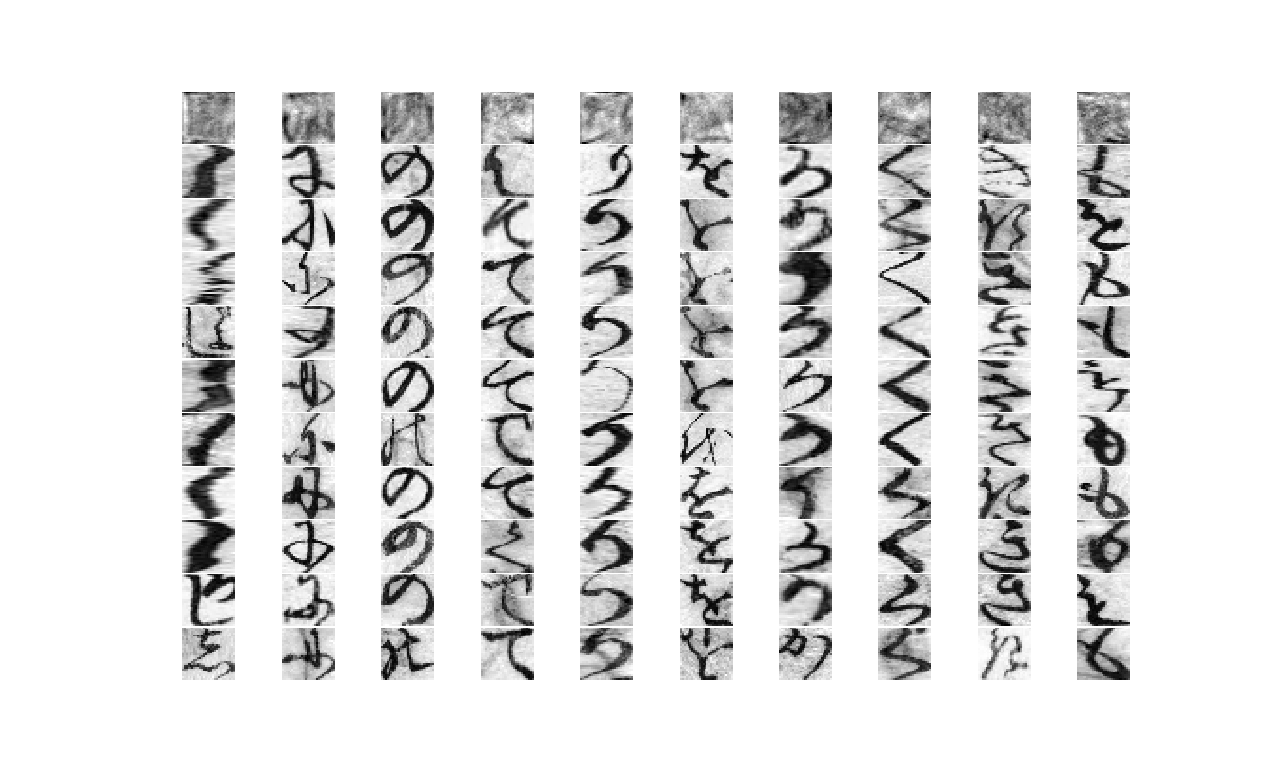
\includegraphics[scale=0.5]{weights.png}}      	
		\end{exercise}
		\begin{exercise}[p=55]{}
			\question{}{}
			\question{}{}
			\question{}{
			train accuracy: 99.995\%\\
			test accuracy: 97.496\%}
			\question{}{When we removed the second convolutional layer, we obtained the following results:\\
			train accuracy: 99.970\%\\
			test accuracy: 96.101\%\\
			We see that while the train accuracy hardly changes, the test accuracy deteriorates more strongly. Therefore we conclude, that removing one layer causes the model to overfit because it loses some ability to generalize.
			}
			\question{}{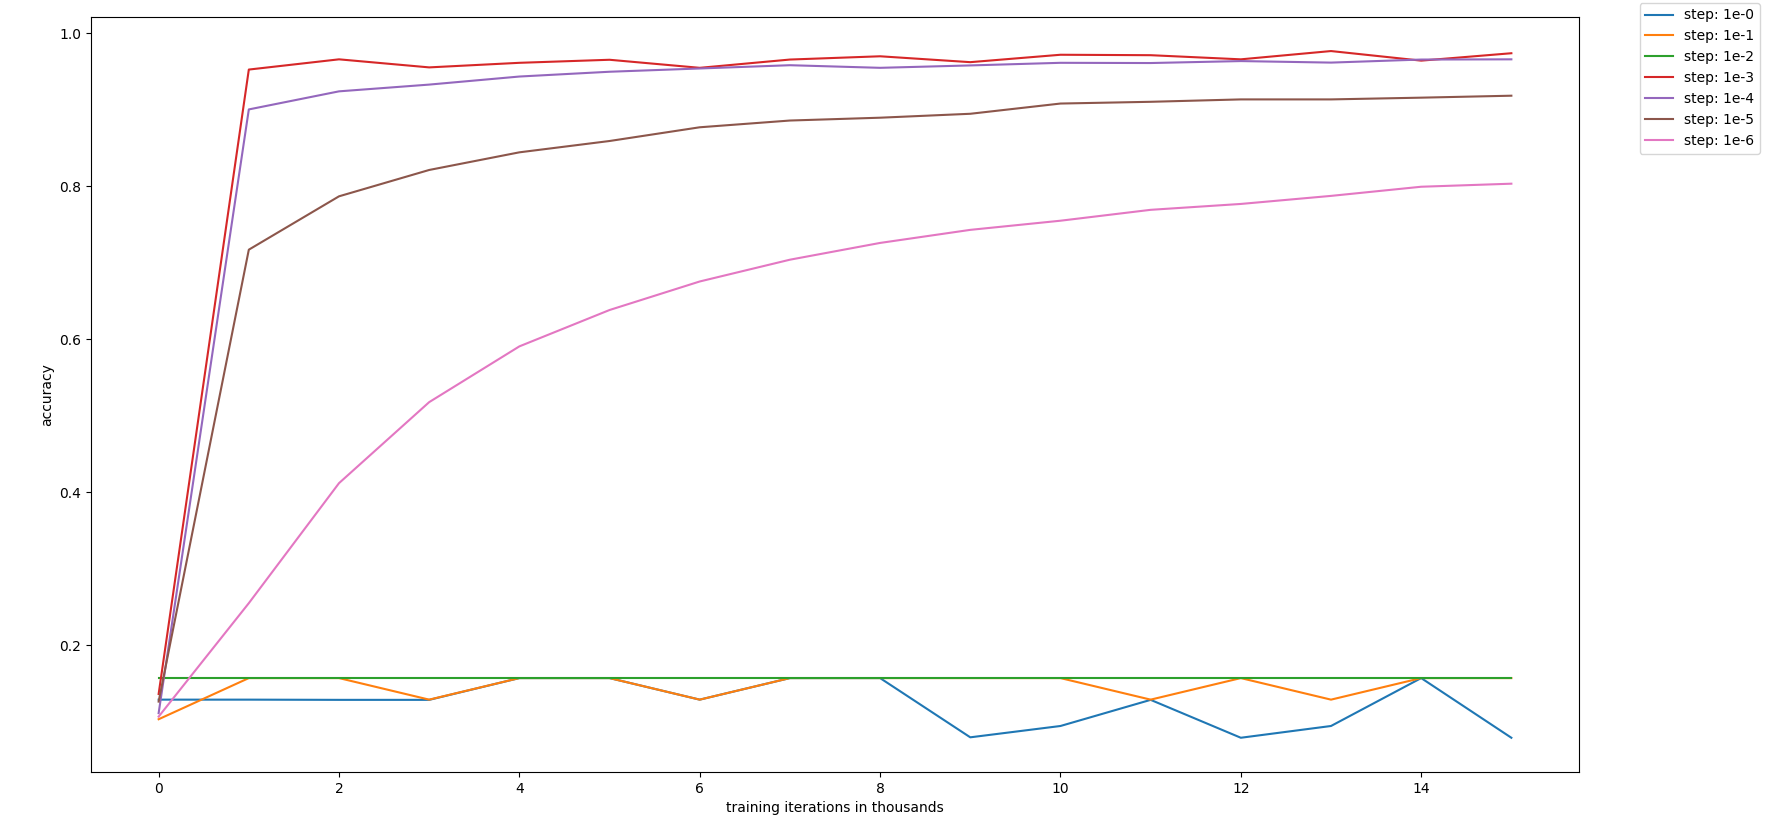
\includegraphics[scale=1.2]{step.png}}
			\question{}{
			size of convolutional layer:\\
			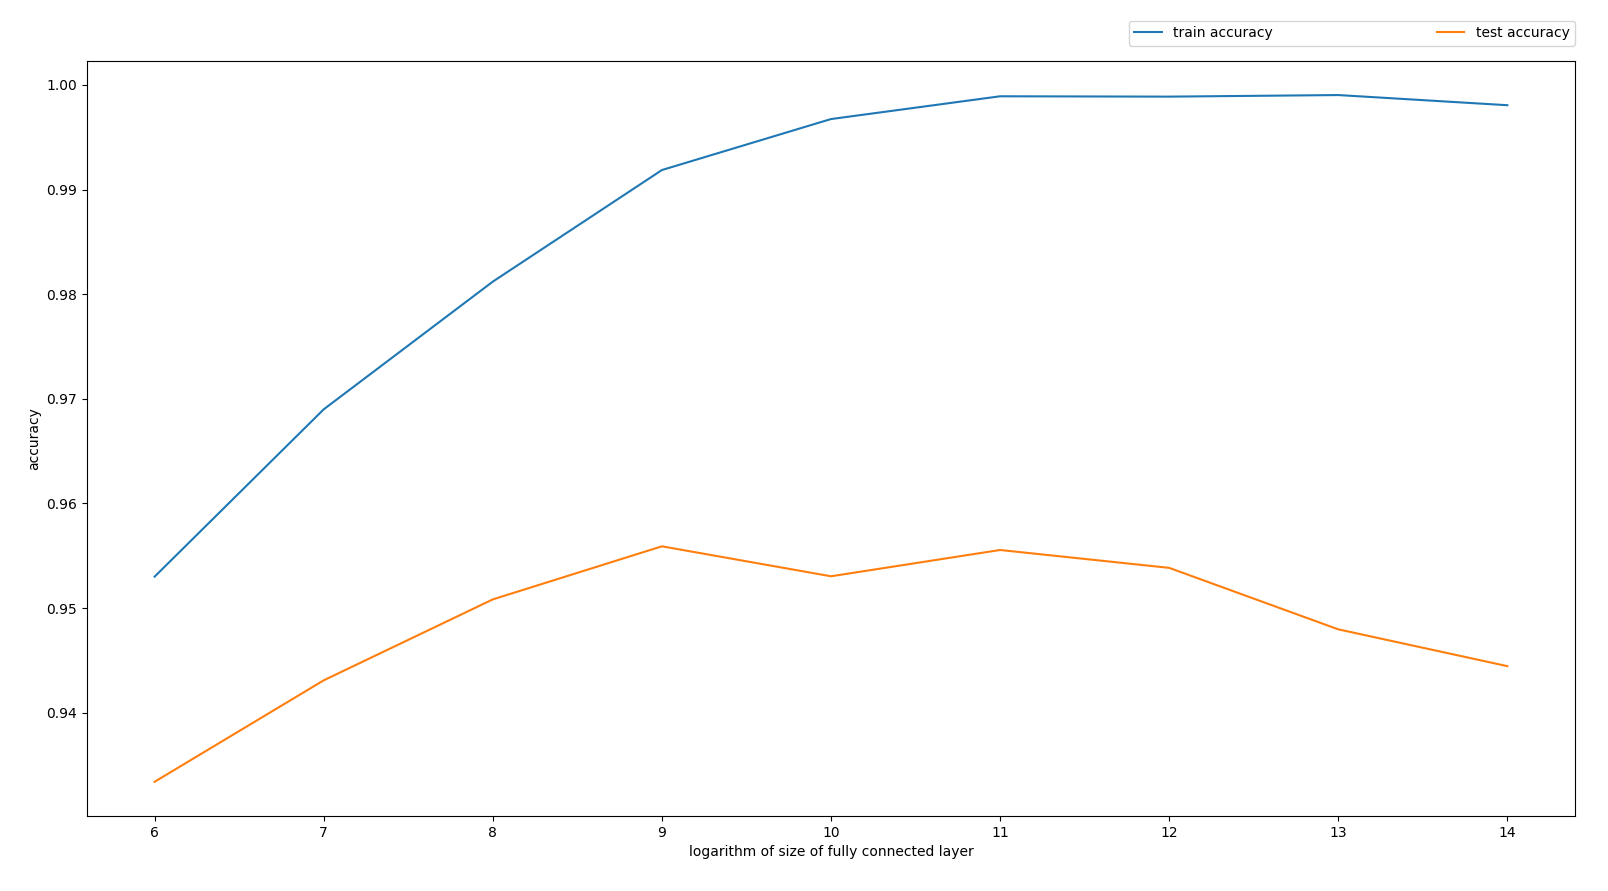
\includegraphics[scale=1.1]{convsize.png}\\
			size of kernels: || number of features in the first convolutional layer:\\
			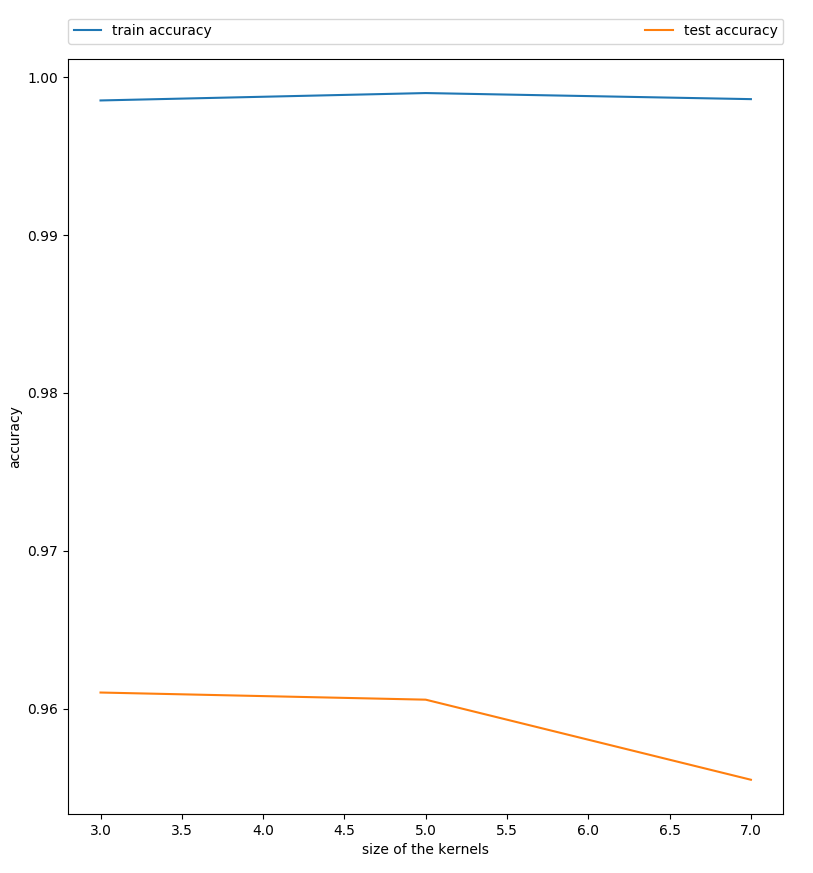
\includegraphics[scale=1.1]{kernelsize.png}
			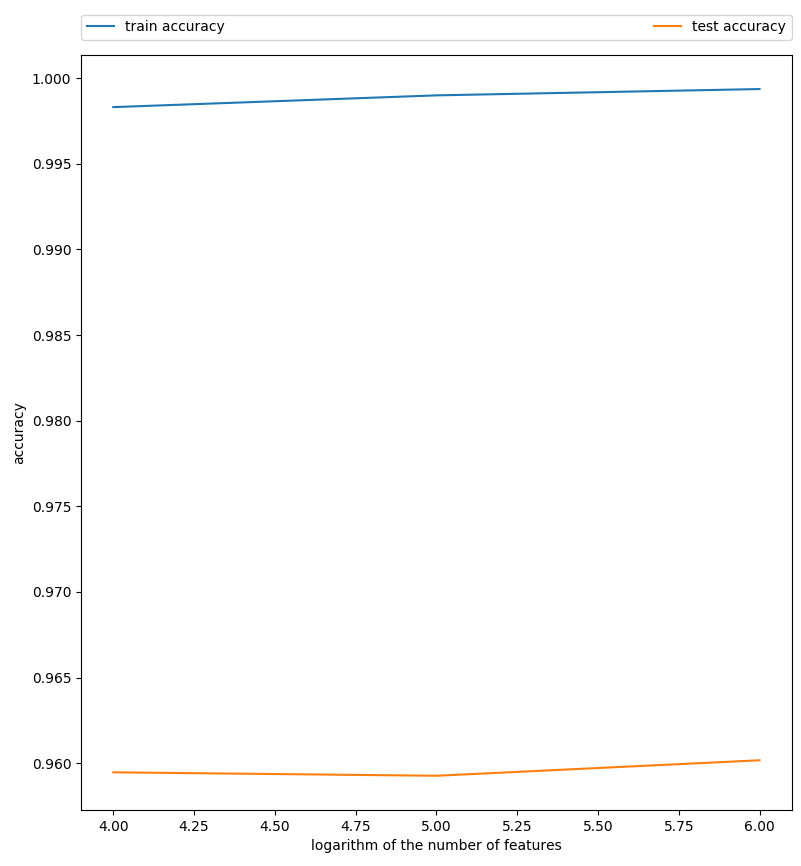
\includegraphics[scale=1.1]{featurecount.png}\\
			}
		\end{exercise}
		\begin{exercise}[p=20]{}
		\question{}{see regression.py}
		\question{}{
		Accuracy for the logistc regression model fully trained on MINIST: 92\%\\
		Accuracy for the convolutional model fully trained on MINIST: 99.7\%\\
		Accuracy when retraining in- and output-weights of the fully connected layer: 99.10\%\\
		Accuracy when only retraining output-weights of the fully connected layer: 97.86\%\\
		\\
		Altough the features were trained on the japanese characters, they could also be used to relatively accurately classify MINIST data even though much less parameters had to be trained.\\
		Considering that the amount of weights you have to train when only retraining output-weights of the fully connected layer is only slightly bigger than the amount of weights in the regression model, it seems way more efficient to retrain the fully connected layer, looking at the difference in achieved accuracy of these two options.\\
		
		}
		\end{exercise}
		\begin{exercise}[p=20]{}
		
		\end{exercise}
		\begin{exercise}[p=20]{}
		
		\end{exercise}
		
		
\end{ukon-infie}
\end{document}
